\chapter{Lecture 8}

%--- 信息 ----
\begin{center}
    讲师:王立威 \qquad
    课程时间:25.Apr.8th \qquad 
    笔记:25.June.8th
\end{center}

\bigskip

来讨论信道编码,动机在于真实世界的信道都是含噪的,噪声会干扰信息的传递致使接收到的信息和发送的信息不完全相同。自然地,我们想要设计一套算法来纠正由噪声引起的错误,这套算法应该包含编码(encoding)和解码(decoding)两部分。

\begin{example}
    一个最简单的想法就是编码时重复三次,解码时取众数。
\end{example}

上面的例子虽然简单,但却内蕴了深刻的思想——解码时将内容映射到最近邻的合理码字. 这里的最近邻使用的是Hamming距离(请自行查阅). 

我们设$M_i$对应的编码是$c_i$(对于所有$1 \le i \le n$),那么有如下定理:
\begin{theorem}
    对于正整数$t > 0$,若对于任意$i\neq j$都有$d_H(c_i,c_j) \ge 2t + 1$,那么这样的编码可以纠正$t$比特的错误. 
\end{theorem}

我现在希望将信息空间映射到编码空间 
\[
\text{Message Space} \quad \{0,1\}^m \quad \quad \longrightarrow \quad \quad
\text{Coding Space} \quad \{0,1\}^n 
\]

现在给定$t,m$,来估计一下$n$的下界. 
\begin{proposition}
    上述条件下,需要满足 
    \[
    2^n \ge 2^m \cdot {\sum_{i=1}^t \binom{n}{i}}
    \]
\end{proposition}
\begin{proof}
统计一下球形邻域$B(x):= \{y:d_H(x,y) \le t\}$的大小,注意到对于任意$i\neq j$,要有$B(c_i)\cap B(c_j) = \varnothing$
\end{proof}

接着来计算其上界。这里我们将目标重述为给定$m$和$ \de \in (0, 1/2)$,找一个尽量小的$n$使得一定存在编码$c_1, c_2, \dots, c_{2^m} \in \{0,1\}^n$使得
\[
d_H(c_i, c_j) \ge \de n , \quad \forall i \neq j
\]

采用概率方法(这是现代组合数学的常用技巧)可以证明如下结论。
\begin{theorem}[Gilbert-Vashamov界]
    如果对于某个常数$c$($c$依赖于$\de$),$n \ge cm$,那么存在一组编码符合条件.
\end{theorem}
\begin{proof}
    由于$c_i, c_j$是独立且均匀地在$\{0,1\}^n$熵采样得到的,所以事实上$d_H(c_i,c_j) \sim B(n, 1/2)$。 根据Chernoff Bound,可以得到 
\[
\Pr \Big[
d_H(c_i, c_j) < \de n  
\Big] < e^{- \ln 2  D(\de \| 1/2) \cdot n} = e^{-O(n)}
\]

根据Union Bound,又有 
\[
\Pr \left[
    \bigcup_{i,j \in [2^m]: i\neq j} d_H(c_i, c_j) < \de n
\right] < \binom{2^m}{2}e^{-O(n)}
\]

所以 
\[
\Pr \Big[
    \forall i\neq j \in [2^m],\ d_H(c_i,c_j) \ge \de n
\Big] \ge 1 - \binom{2^m}{2}e^{-O(n)}
\]

我们只需要上式右侧大于0即可,化简可以得到这需要 
\[
n \ge \Omega(m)
\]

也就证明了结论。事实上,这个$c$可以取成$\dfrac{2}{D(\de \| \frac 12)}$。
\end{proof}

总结一下设计一套纠错码的流程 
\begin{enumerate}
    \item 首先要设计一组码字$c_1,c_2,\dots, c_N$,使得它们彼此Hamming充分大(达到预期纠错的能力)。
    \item 然后给出一个编码算法,将消息映射到码字。
    \item 最后给出解码算法,找到接受消息最近的码字。
\end{enumerate}

这里的第3步比较特殊,一般$m$可以来到上百的量级,码字计算会来到2的上百次方量级,朴素寻找最近邻码字是不现实的。我们必须要考虑编码和解码的计算复杂度。 这部分也是该领域着重努力的方向。 

一个最早期的做法是Hamming码

% \begin{figure}[H]
%     \centering
%     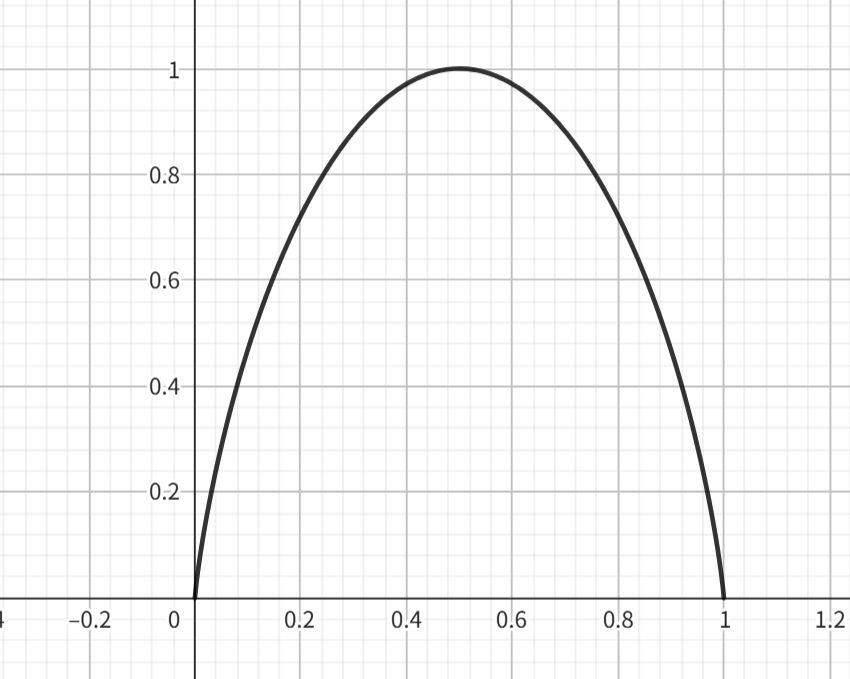
\includegraphics[width=.6\textwidth]{images/c2_1.png}
%     \caption{$H=x\log 1/x + (1-x)\log 1/(1-x)$的图像}
% \end{figure}